\documentclass[tikz,svgnames]{standalone}

\begin{document}

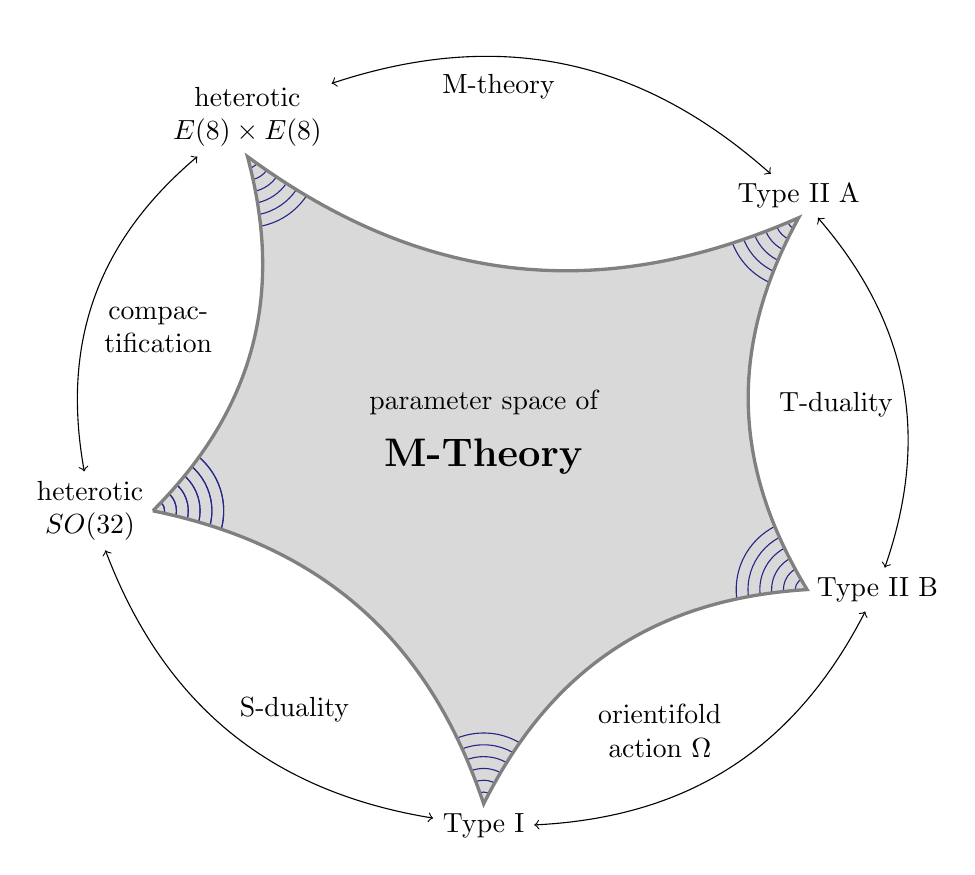
\begin{tikzpicture}

  \node (so32) [align=center] at (-5,-1) {heterotic\\$SO(32)$};
  \node (e8e8) [align=center] at (-3,4) {heterotic\\$E(8) \times E(8)$};
  \node (tiia) [align=center] at (4,3) {Type II A};
  \node (tiib) [align=center] at (5,-2) {Type II B};
  \node (ti) [align=center] at (0,-5) {Type I};

  \draw[bend left,<->]  (so32) to node [below right,align=center] {compac-\\tification} (e8e8);
  \draw[bend left,<->]  (e8e8) to node [below left] {M-theory} (tiia);
  \draw[bend left,<->]  (tiia) to node [below left] {T-duality} (tiib);
  \draw[bend left,<->]  (tiib) to node [above left,align=center] {orientifold\\action $\Omega$} (ti);
  \draw[bend left,<->]  (ti) to node [above right] {S-duality} (so32);

  \begin{scope}
    \clip[bend right]
    (so32.east)
    to (e8e8.south)
    to (tiia.south)
    to (tiib.west)
    to (ti.north)
    to (so32.east);
    \foreach \c in {so32.east,e8e8.south,tiia.south,tiib.west,ti.north,so32.east}{%
        \foreach \r in {1,...,6}{%
            \draw[DarkBlue] (\c) circle (\r*0.15cm);
          }
      }
  \end{scope}

  \draw[bend right,very thick,gray,fill,fill opacity=0.3]  (so32.east) to (e8e8.south) to (tiia.south) to (tiib.west) to (ti.north) to (so32.east);

  \node (mth) [align=center] at (0,0) {parameter space of\\[2ex]{\Large \textbf{M-Theory}}};

\end{tikzpicture}

\end{document}